\documentclass[]{book}
\usepackage{lmodern}
\usepackage{amssymb,amsmath}
\usepackage{ifxetex,ifluatex}
\usepackage{fixltx2e} % provides \textsubscript
\ifnum 0\ifxetex 1\fi\ifluatex 1\fi=0 % if pdftex
  \usepackage[T1]{fontenc}
  \usepackage[utf8]{inputenc}
\else % if luatex or xelatex
  \ifxetex
    \usepackage{mathspec}
  \else
    \usepackage{fontspec}
  \fi
  \defaultfontfeatures{Ligatures=TeX,Scale=MatchLowercase}
\fi
% use upquote if available, for straight quotes in verbatim environments
\IfFileExists{upquote.sty}{\usepackage{upquote}}{}
% use microtype if available
\IfFileExists{microtype.sty}{%
\usepackage[]{microtype}
\UseMicrotypeSet[protrusion]{basicmath} % disable protrusion for tt fonts
}{}
\PassOptionsToPackage{hyphens}{url} % url is loaded by hyperref
\usepackage[unicode=true]{hyperref}
\hypersetup{
            pdftitle={Inferential Statistics Notes},
            pdfauthor={KS},
            pdfborder={0 0 0},
            breaklinks=true}
\urlstyle{same}  % don't use monospace font for urls
\usepackage{natbib}
\bibliographystyle{apalike}
\usepackage{color}
\usepackage{fancyvrb}
\newcommand{\VerbBar}{|}
\newcommand{\VERB}{\Verb[commandchars=\\\{\}]}
\DefineVerbatimEnvironment{Highlighting}{Verbatim}{commandchars=\\\{\}}
% Add ',fontsize=\small' for more characters per line
\usepackage{framed}
\definecolor{shadecolor}{RGB}{248,248,248}
\newenvironment{Shaded}{\begin{snugshade}}{\end{snugshade}}
\newcommand{\KeywordTok}[1]{\textcolor[rgb]{0.13,0.29,0.53}{\textbf{#1}}}
\newcommand{\DataTypeTok}[1]{\textcolor[rgb]{0.13,0.29,0.53}{#1}}
\newcommand{\DecValTok}[1]{\textcolor[rgb]{0.00,0.00,0.81}{#1}}
\newcommand{\BaseNTok}[1]{\textcolor[rgb]{0.00,0.00,0.81}{#1}}
\newcommand{\FloatTok}[1]{\textcolor[rgb]{0.00,0.00,0.81}{#1}}
\newcommand{\ConstantTok}[1]{\textcolor[rgb]{0.00,0.00,0.00}{#1}}
\newcommand{\CharTok}[1]{\textcolor[rgb]{0.31,0.60,0.02}{#1}}
\newcommand{\SpecialCharTok}[1]{\textcolor[rgb]{0.00,0.00,0.00}{#1}}
\newcommand{\StringTok}[1]{\textcolor[rgb]{0.31,0.60,0.02}{#1}}
\newcommand{\VerbatimStringTok}[1]{\textcolor[rgb]{0.31,0.60,0.02}{#1}}
\newcommand{\SpecialStringTok}[1]{\textcolor[rgb]{0.31,0.60,0.02}{#1}}
\newcommand{\ImportTok}[1]{#1}
\newcommand{\CommentTok}[1]{\textcolor[rgb]{0.56,0.35,0.01}{\textit{#1}}}
\newcommand{\DocumentationTok}[1]{\textcolor[rgb]{0.56,0.35,0.01}{\textbf{\textit{#1}}}}
\newcommand{\AnnotationTok}[1]{\textcolor[rgb]{0.56,0.35,0.01}{\textbf{\textit{#1}}}}
\newcommand{\CommentVarTok}[1]{\textcolor[rgb]{0.56,0.35,0.01}{\textbf{\textit{#1}}}}
\newcommand{\OtherTok}[1]{\textcolor[rgb]{0.56,0.35,0.01}{#1}}
\newcommand{\FunctionTok}[1]{\textcolor[rgb]{0.00,0.00,0.00}{#1}}
\newcommand{\VariableTok}[1]{\textcolor[rgb]{0.00,0.00,0.00}{#1}}
\newcommand{\ControlFlowTok}[1]{\textcolor[rgb]{0.13,0.29,0.53}{\textbf{#1}}}
\newcommand{\OperatorTok}[1]{\textcolor[rgb]{0.81,0.36,0.00}{\textbf{#1}}}
\newcommand{\BuiltInTok}[1]{#1}
\newcommand{\ExtensionTok}[1]{#1}
\newcommand{\PreprocessorTok}[1]{\textcolor[rgb]{0.56,0.35,0.01}{\textit{#1}}}
\newcommand{\AttributeTok}[1]{\textcolor[rgb]{0.77,0.63,0.00}{#1}}
\newcommand{\RegionMarkerTok}[1]{#1}
\newcommand{\InformationTok}[1]{\textcolor[rgb]{0.56,0.35,0.01}{\textbf{\textit{#1}}}}
\newcommand{\WarningTok}[1]{\textcolor[rgb]{0.56,0.35,0.01}{\textbf{\textit{#1}}}}
\newcommand{\AlertTok}[1]{\textcolor[rgb]{0.94,0.16,0.16}{#1}}
\newcommand{\ErrorTok}[1]{\textcolor[rgb]{0.64,0.00,0.00}{\textbf{#1}}}
\newcommand{\NormalTok}[1]{#1}
\usepackage{longtable,booktabs}
% Fix footnotes in tables (requires footnote package)
\IfFileExists{footnote.sty}{\usepackage{footnote}\makesavenoteenv{long table}}{}
\usepackage{graphicx,grffile}
\makeatletter
\def\maxwidth{\ifdim\Gin@nat@width>\linewidth\linewidth\else\Gin@nat@width\fi}
\def\maxheight{\ifdim\Gin@nat@height>\textheight\textheight\else\Gin@nat@height\fi}
\makeatother
% Scale images if necessary, so that they will not overflow the page
% margins by default, and it is still possible to overwrite the defaults
% using explicit options in \includegraphics[width, height, ...]{}
\setkeys{Gin}{width=\maxwidth,height=\maxheight,keepaspectratio}
\IfFileExists{parskip.sty}{%
\usepackage{parskip}
}{% else
\setlength{\parindent}{0pt}
\setlength{\parskip}{6pt plus 2pt minus 1pt}
}
\setlength{\emergencystretch}{3em}  % prevent overfull lines
\providecommand{\tightlist}{%
  \setlength{\itemsep}{0pt}\setlength{\parskip}{0pt}}
\setcounter{secnumdepth}{5}
% Redefines (sub)paragraphs to behave more like sections
\ifx\paragraph\undefined\else
\let\oldparagraph\paragraph
\renewcommand{\paragraph}[1]{\oldparagraph{#1}\mbox{}}
\fi
\ifx\subparagraph\undefined\else
\let\oldsubparagraph\subparagraph
\renewcommand{\subparagraph}[1]{\oldsubparagraph{#1}\mbox{}}
\fi

% set default figure placement to htbp
\makeatletter
\def\fps@figure{htbp}
\makeatother

\usepackage{booktabs}
\usepackage{amsthm}
\makeatletter
\def\thm@space@setup{%
  \thm@preskip=8pt plus 2pt minus 4pt
  \thm@postskip=\thm@preskip
}
\makeatother

\title{Inferential Statistics Notes}
\author{KS}
\date{2020-07-04}

\begin{document}
\maketitle

{
\setcounter{tocdepth}{1}
\tableofcontents
}
\chapter{Prerequisites}\label{prerequisites}

This is a \emph{sample} book written in \textbf{Markdown}. You can use
anything that Pandoc's Markdown supports, e.g., a math equation
\(a^2 + b^2 = c^2\).

The \textbf{bookdown} package can be installed from CRAN or Github:

\begin{Shaded}
\begin{Highlighting}[]
\KeywordTok{install.packages}\NormalTok{(}\StringTok{"bookdown"}\NormalTok{)}
\CommentTok{# or the development version}
\CommentTok{# devtools::install_github("rstudio/bookdown")}
\end{Highlighting}
\end{Shaded}

Remember each Rmd file contains one and only one chapter, and a chapter
is defined by the first-level heading \texttt{\#}.

To compile this example to PDF, you need XeLaTeX. You are recommended to
install TinyTeX (which includes XeLaTeX):
\url{https://yihui.name/tinytex/}.

\chapter{Central Limit Theorem(CLT) and Sampling}\label{clt}

\section{Chapter Summary}\label{chapter-summary}

\begin{figure}

{\centering 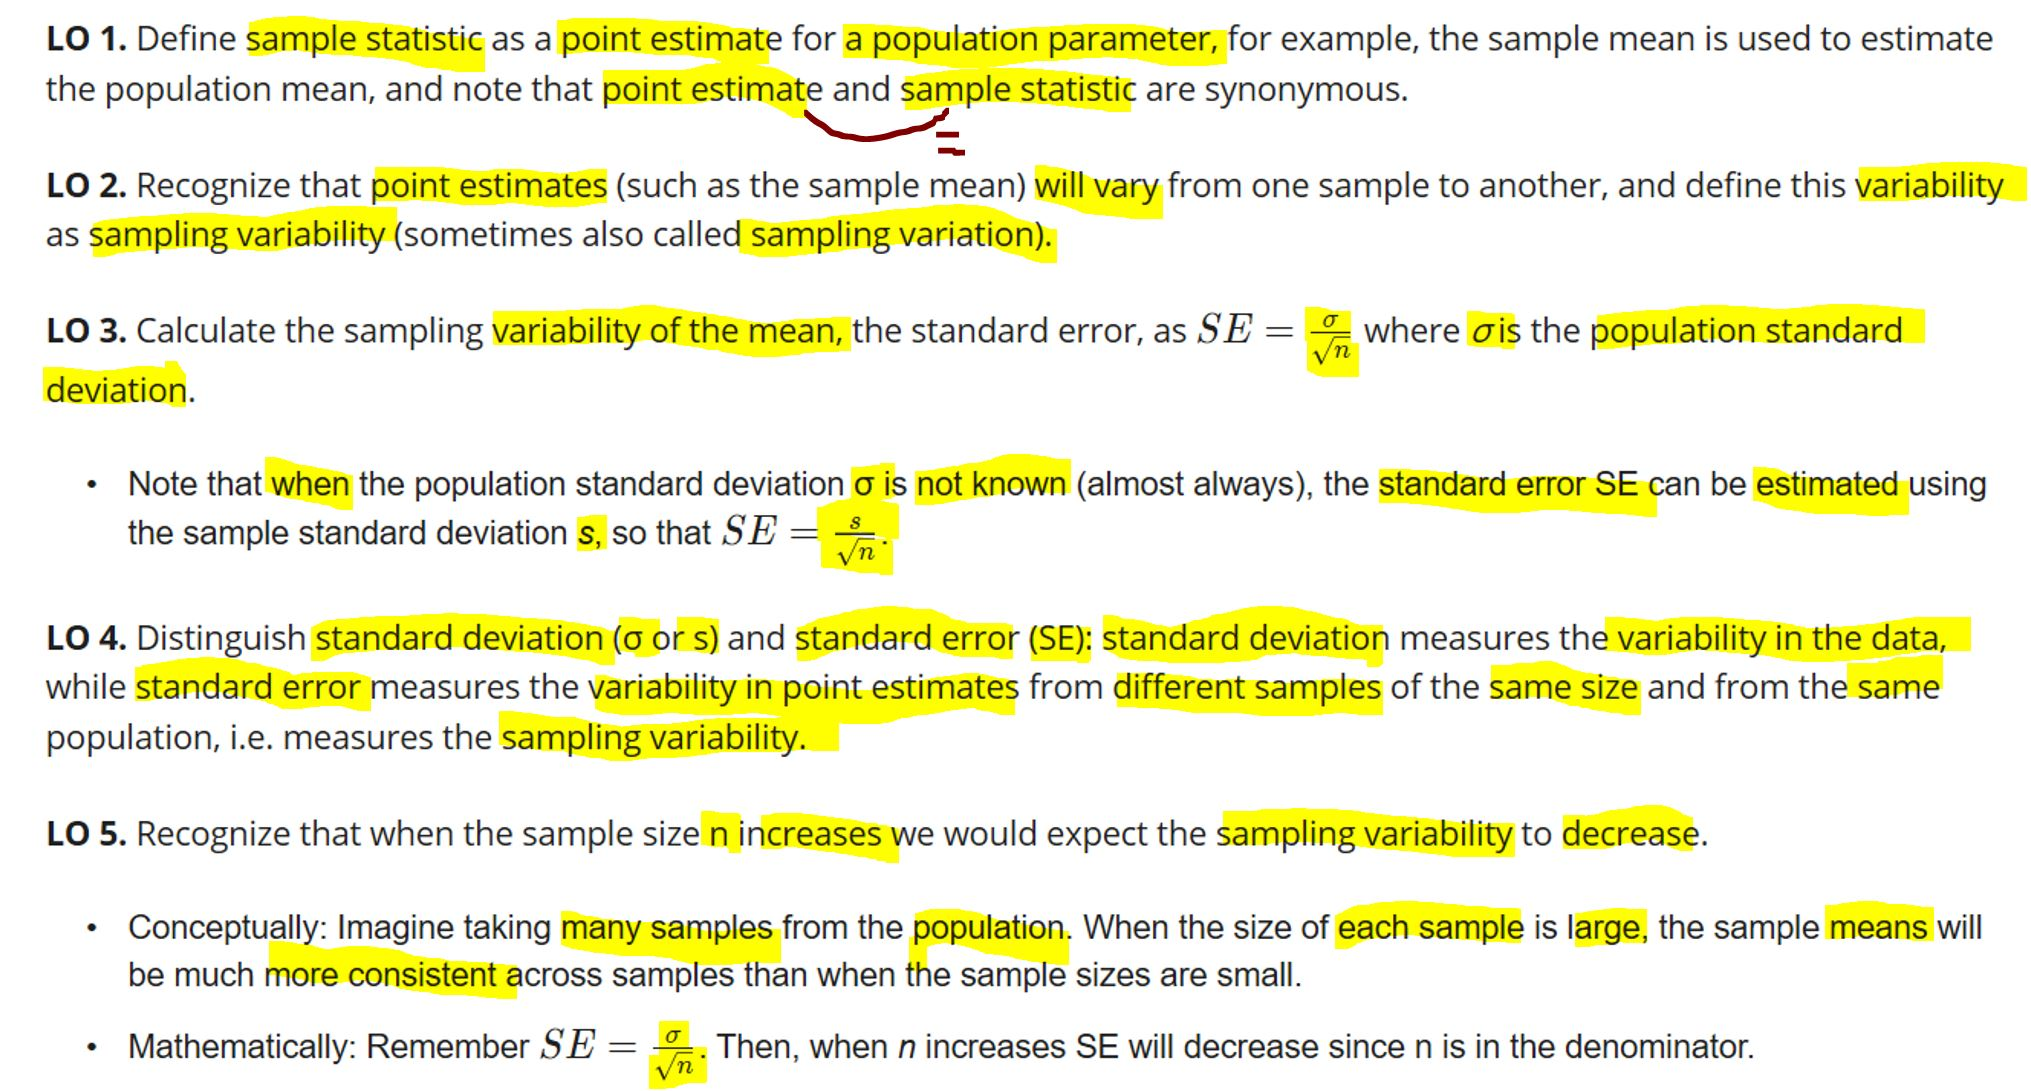
\includegraphics[width=0.8\linewidth]{graphs/1-1} 

}

\caption{Chapter Summary}\label{fig:chap1-summary-fig}
\end{figure}

由于通常不太可能直接获得population
parameter(如全国所有人身高的平均值)因此通常使用sample statistics/point
estimates来约等于或者估算population parameter

在这个例子中,也可以观察到在计算sample
statistics时,每一组sample的平均值都不太一样,之后要计算这些平均值的standard
deviation

\begin{figure}

{\centering 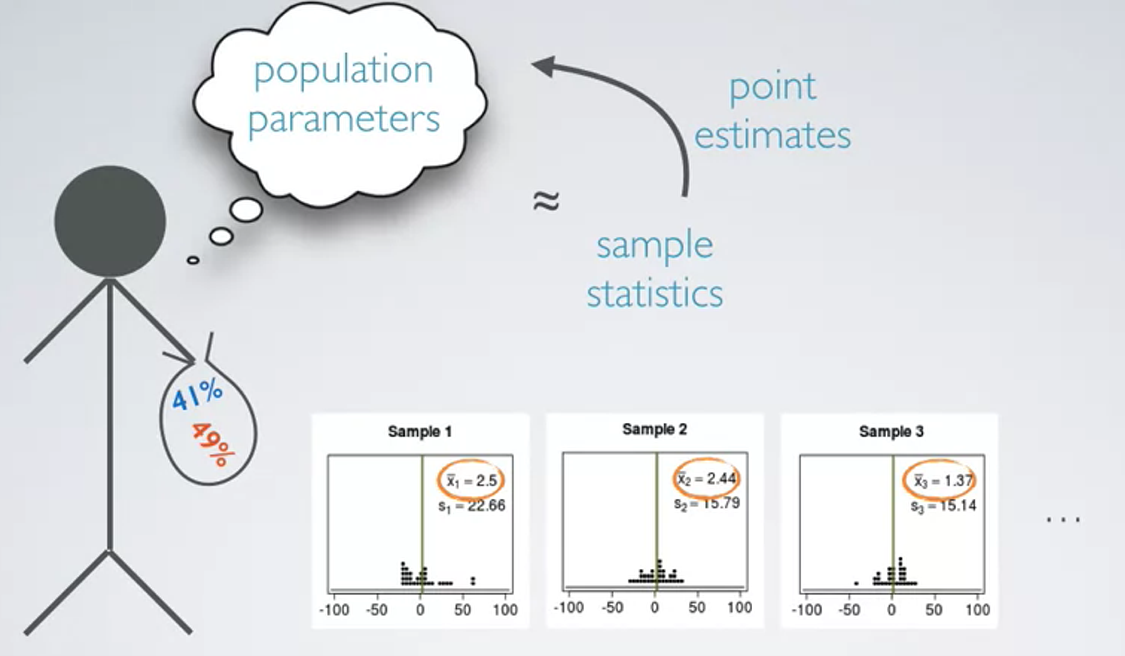
\includegraphics[width=0.8\linewidth]{graphs/1-2} 

}

\caption{Introduction}\label{fig:fig1}
\end{figure}

\section{Sampling Distribution 与 Sampling
Distribution}\label{sampling-distribution-ux4e0e-sampling-distribution}

Sample distribution 和sampling distribution看上去相似但不是同一个意思;

Sample distribution:

\begin{itemize}
\tightlist
\item
  Sample distribution是The distributions of the observations with in
  each sample
\item
  sample distribution的observation是individual(比如说people/case)
\end{itemize}

Sampling distribution:

\begin{itemize}
\tightlist
\item
  Sampling distribution是the distribution of the sample statistics
\item
  sampling distribution的observation是sampled statistics
\end{itemize}

\begin{figure}

{\centering 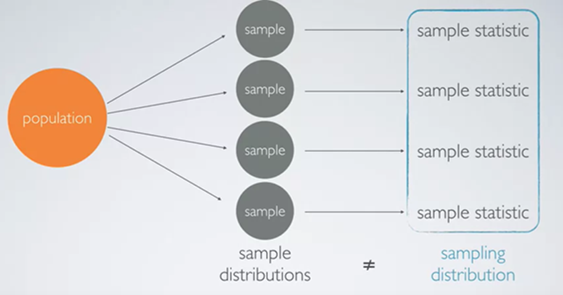
\includegraphics[width=0.8\linewidth]{graphs/1-3} 

}

\caption{Sampling vs. sample distribution}\label{fig:fig3}
\end{figure}

\section{Standard Error}\label{standard-error}

这里在计算全美的平均身高时:

\begin{itemize}
\tightlist
\item
  μ代表population mean
\item
  σ代表population standard deviation
\end{itemize}

但其实每个state的standard
deviation会比population的SD要低的(因为人口基数的不同有的state可能人都高,SD小,但整体全国就会包含个子高的state和个子矮的state,因此SD一定会更高一些-?)

Standard error: the standard deviation of sample mean

\begin{itemize}
\tightlist
\item
  N(这里的N表示sample size)越大,Standard error越小
\end{itemize}

\begin{figure}

{\centering 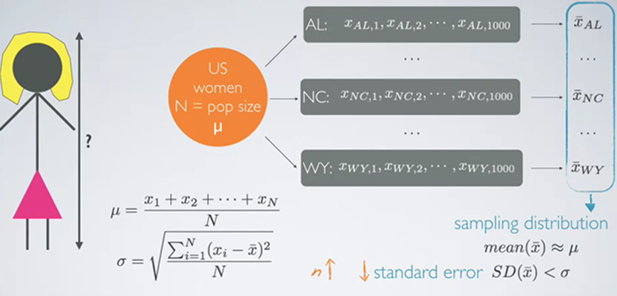
\includegraphics[width=0.8\linewidth]{graphs/1-4} 

}

\caption{Standard error}\label{fig:fig4}
\end{figure}

\section{Central Limit Theorem(CLT)}\label{central-limit-theoremclt}

\textbf{定义}

sample
statistics(如每个sample的mean)的分布应该是正态分布,以population
mean作为中心,并以population SD/根号下sample size作为SE

正常来说应该用population 的SD除根号下sample
size,但通常不太能获取population SD,所以也一般用sample
SD来估计population SD,但这里的sample
SD指的是每次取得的单个sample而不是所有sample之和

\textbf{条件}

\begin{enumerate}
\def\labelenumi{\arabic{enumi}.}
\tightlist
\item
  所有的sample选取要保证互相独立
\end{enumerate}

\begin{itemize}
\tightlist
\item
  可以是random sample/assignment
\item
  如果是无replacement 的取样,应该保证sample size
  N要小于10\%的population(也就是说这种情况下 sample
  size要小一点会好一些,保证sample之间可以相互独立,size太大的话容易收集到具有相似属性的人,如兄弟姐妹家庭等,导致不够independent)
\end{itemize}

\begin{enumerate}
\def\labelenumi{\arabic{enumi}.}
\setcounter{enumi}{1}
\tightlist
\item
  要保证原本整体的population要不然是正态分布,要不然population是skewed并且sample
  size是足够大的(即sample size大于30)
\end{enumerate}

\begin{itemize}
\tightlist
\item
  如果population 不是normal distribution,那么population
  越skewed,需要的sample size就要越大
\item
  如果population是highly right skewed, 选取的sample
  size又很少,那么sample mean的distribution也会是right
  skewed,只有sample size大到一定程度,才能变成normalization
\end{itemize}

\begin{figure}

{\centering 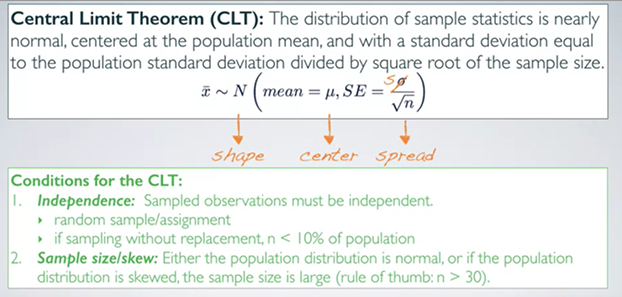
\includegraphics[width=0.8\linewidth]{graphs/1-5} 

}

\caption{Standard error}\label{fig:fig5}
\end{figure}

\textbf{Exercise}

\begin{itemize}
\tightlist
\item
  用于直接visualize各种distribution的\href{https://gallery.shinyapps.io/CLT_mean/}{website}
\item
  例题1:
\end{itemize}

\begin{figure}

{\centering 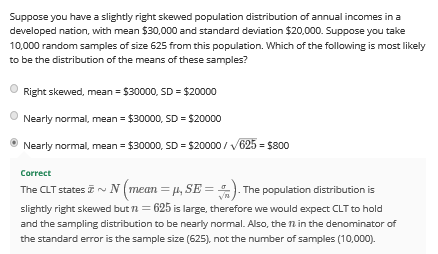
\includegraphics[width=0.8\linewidth]{graphs/1-6} 

}

\caption{Ex 1}\label{fig:fig6}
\end{figure}

\begin{itemize}
\tightlist
\item
  例题2:
\end{itemize}

\begin{figure}

{\centering 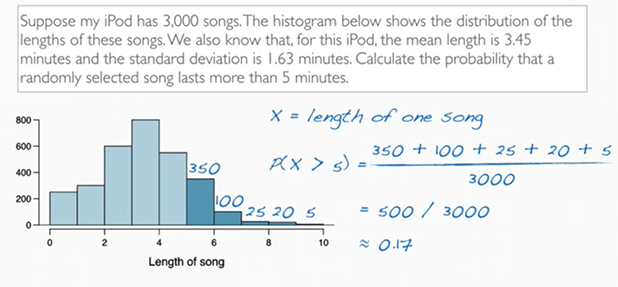
\includegraphics[width=0.8\linewidth]{graphs/1-7} 

}

\caption{Ex 2}\label{fig:fig7}
\end{figure}

这里并不能直接用Z-score
来计算length大于5的歌曲的概率,因为只有在population distribution为normal
distribution的时候才可以这么计算。

这里的分布是right skewed,因此可以利用histogram
来粗略估计,从而得到0.17的概率。

\begin{itemize}
\tightlist
\item
  例题3:
\end{itemize}

\begin{figure}

{\centering 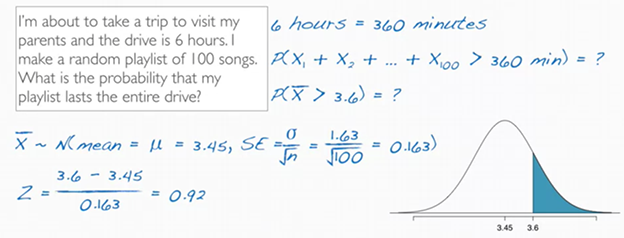
\includegraphics[width=0.8\linewidth]{graphs/1-8} 

}

\caption{Ex 2}\label{fig:fig81}
\end{figure}\begin{figure}

{\centering 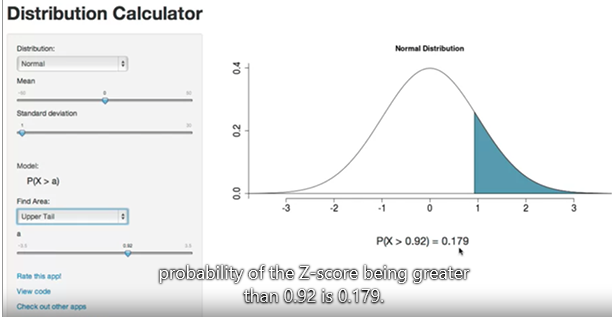
\includegraphics[width=0.8\linewidth]{graphs/1-9} 

}

\caption{Ex 2}\label{fig:fig82}
\end{figure}

在这个情况下,要计算probability的时候,我们不是要求每首歌都长于3.6min,而是要求这100首歌的总时长大于360mins,即sample
mean of those 100 songs \textgreater{} 3.6.

基于CLT,可以知道这些歌的sample mean会是normal分布,
因此可以计算z-score。

\begin{itemize}
\tightlist
\item
  这里计算Z的时候要除以standard deviation of sample mean(即SE, 0.163),
  而不是population
  SD(1.63),因为这里讨论的对象并不是单首歌的时长,而是平均每首歌的sample
  mean, 因此要用SE。
\item
  最后用table或者各种方法,找到对应z-score为0.92的probability,即0.179
\end{itemize}

\begin{quote}
Both in a population and in one, one sample, the observations are still
individual observations, so not sample means. (?)
\end{quote}

即如果将一个sample组中的所有数据拿出来,这样还是会体现出原本population的分布情况,而不是sample
mean的分布情况。

\begin{itemize}
\tightlist
\item
  例题4:
\end{itemize}

\begin{figure}

{\centering 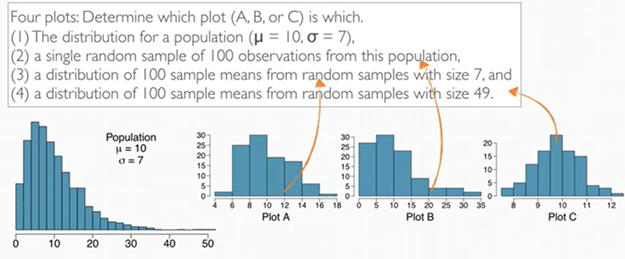
\includegraphics[width=0.8\linewidth]{graphs/1-10} 

}

\caption{Ex 3}\label{fig:fig10}
\end{figure}

\begin{itemize}
\tightlist
\item
  这里可以先选出选项4对应plot
  C,因为选项4可以判断,由于本身population是right-skewed,因此当sample
  size足够大的时候,sample mean应该是normal distribution
\item
  在剩下的两个中,由于选项2描述的a single random sample of 100
  observations,
  即一组sample的数据,其本质还是population的分布,所以仍然会显示right-skewed
\item
  而选项3描述的是一个sample size比较小的sample
  mean的distribution,因此会显示出一些normal
  distribution的样子,但也会显示一些right-skewed的样子
\end{itemize}

\chapter{Confidence Intervals}\label{conf-int}

\section{Chapter Summary}\label{chapter-summary}

\begin{figure}

{\centering 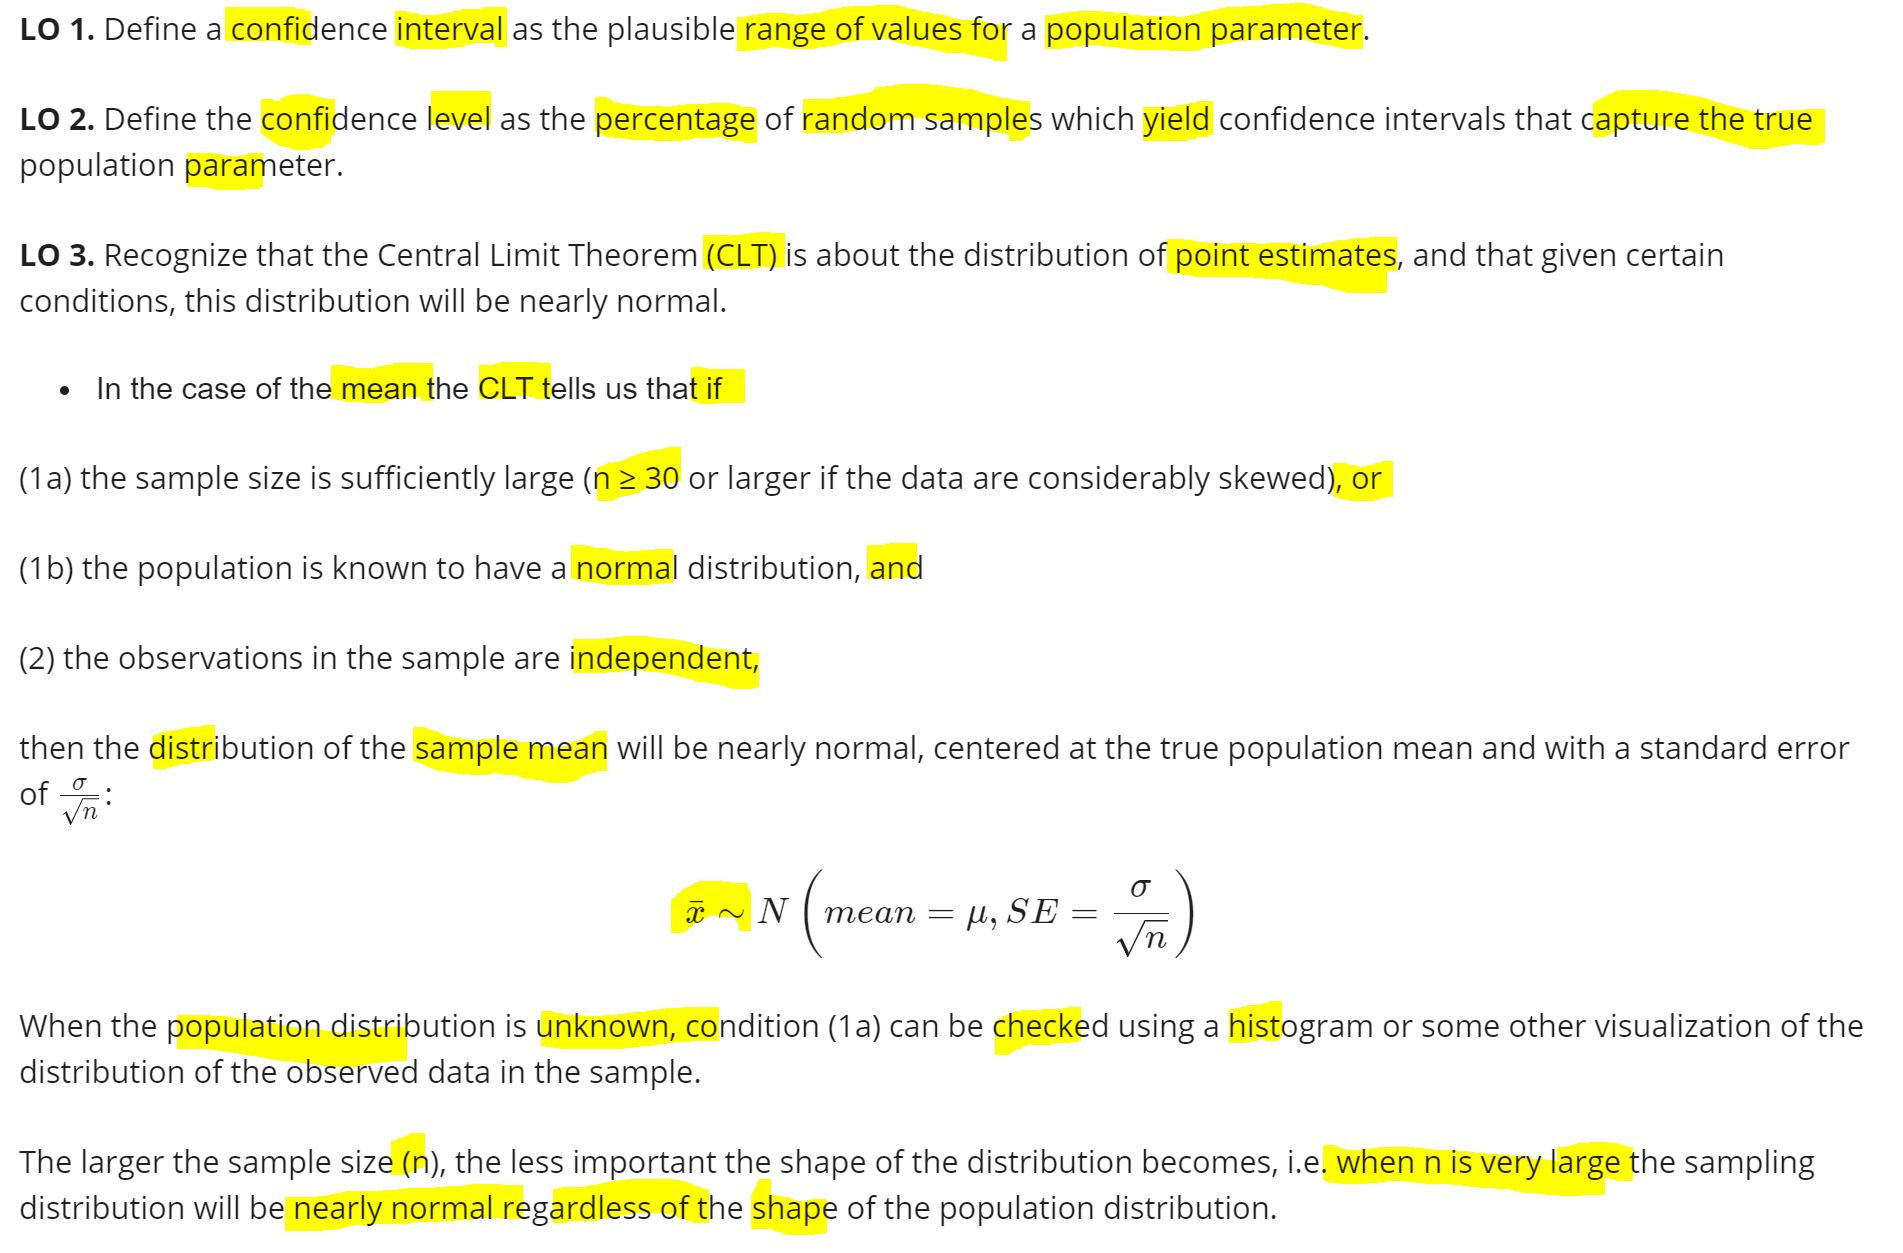
\includegraphics[width=0.8\linewidth]{graphs/2-1} 

}

\caption{Chapter Summary}\label{fig:chap2-summary-fig1}
\end{figure}\begin{figure}

{\centering 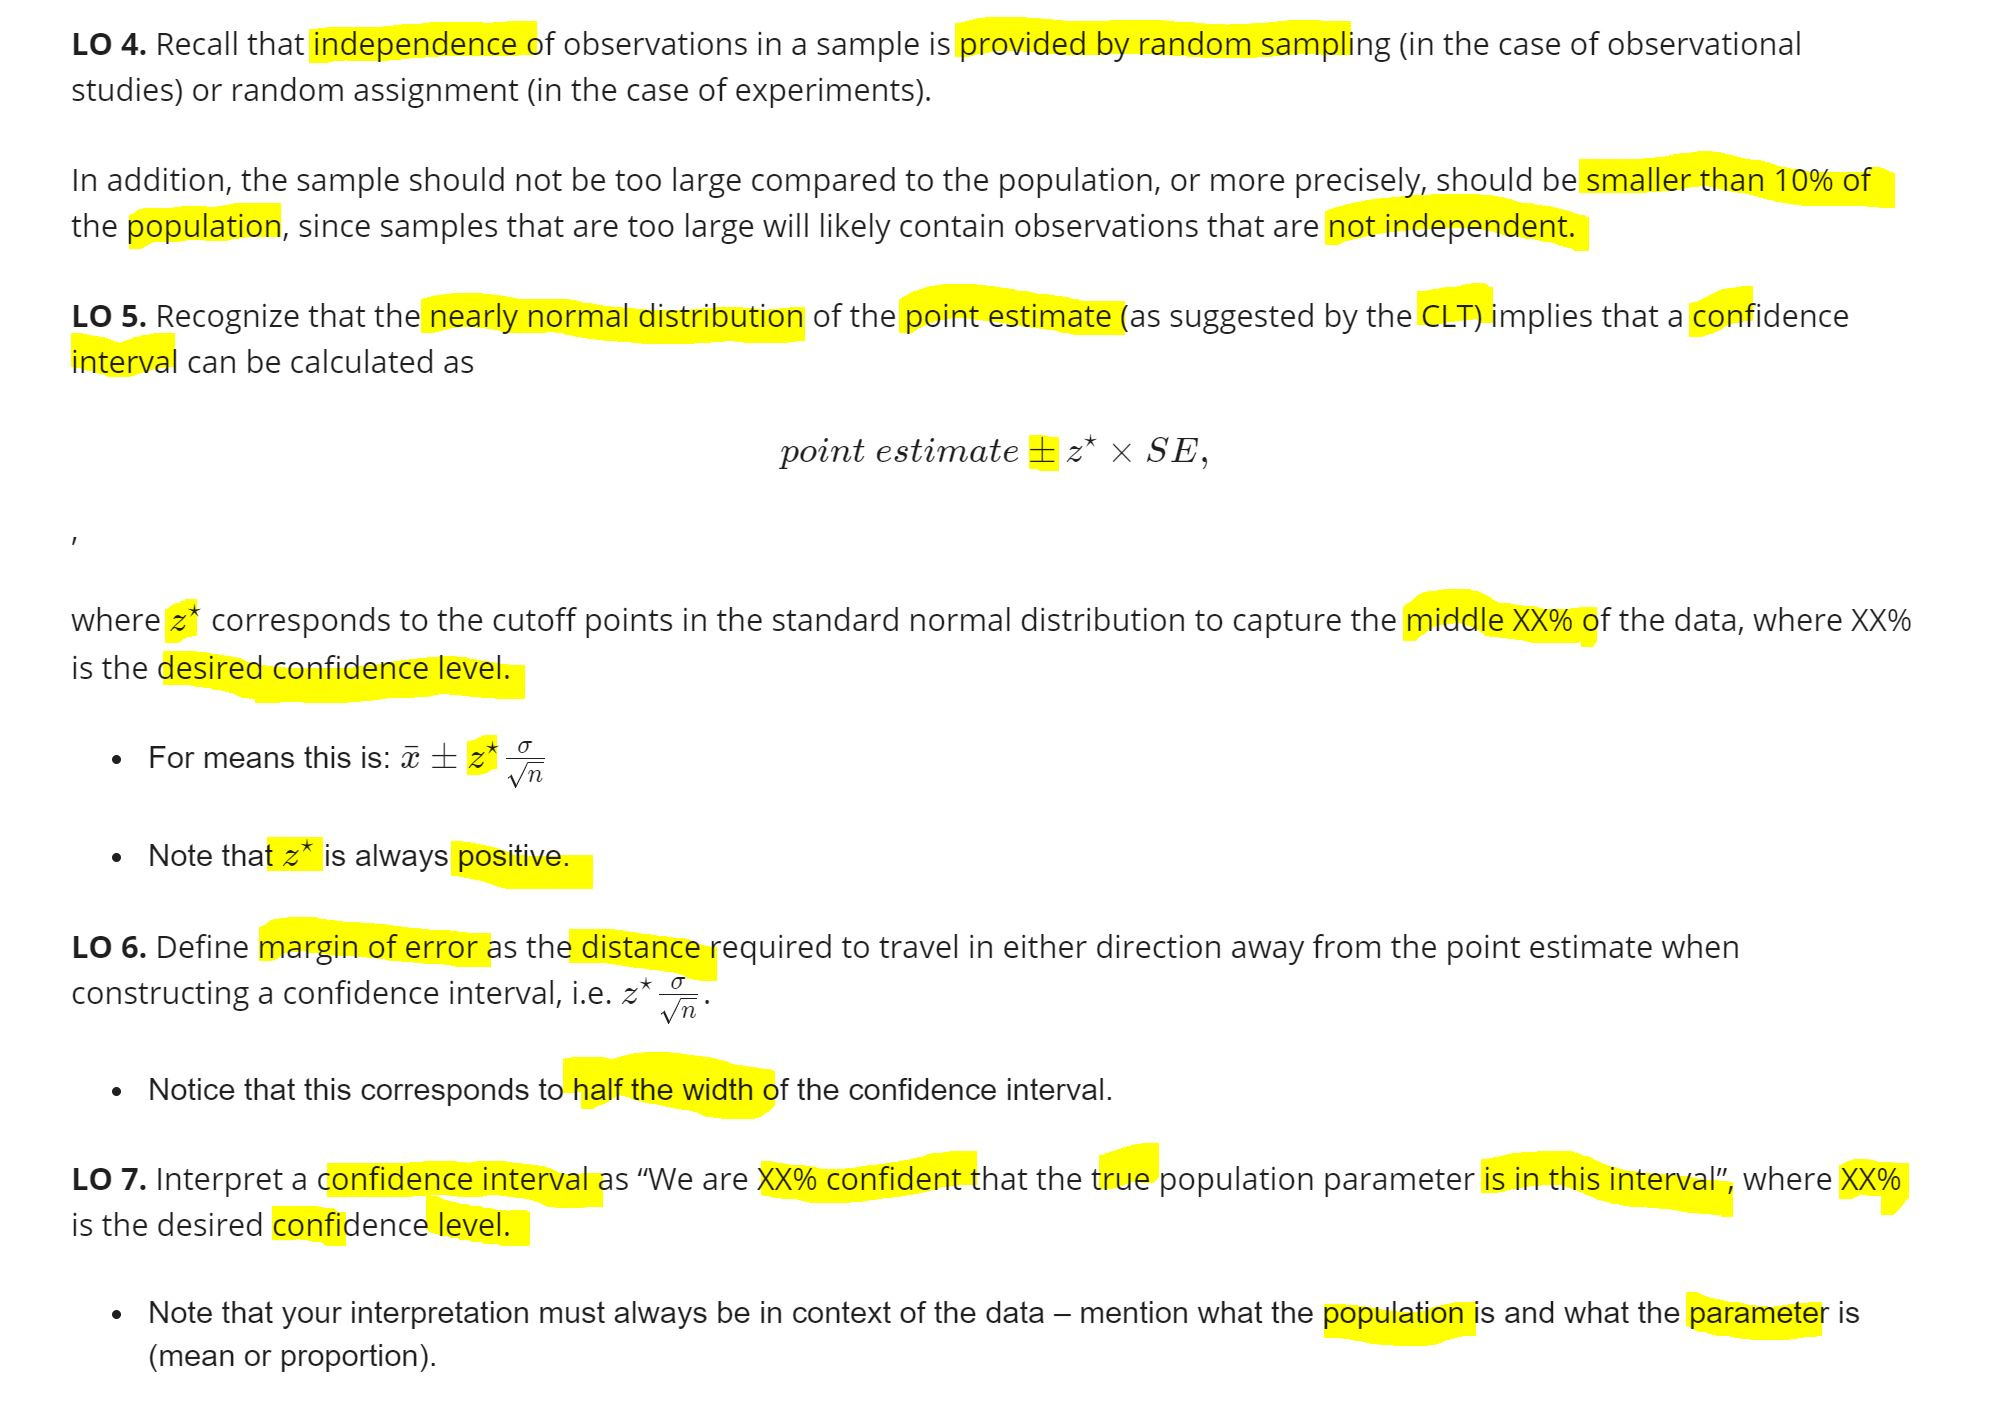
\includegraphics[width=0.8\linewidth]{graphs/2-2} 

}

\caption{Chapter Summary}\label{fig:chap2-summary-fig2}
\end{figure}

\section{Interval Estimate}\label{interval-estimate}

当我们希望对一个population的parameter(如mean)做出预测的时候,
通过预测这个parameter是否在一个range之中的方式更好(而不是point
estimate)

\begin{figure}

{\centering 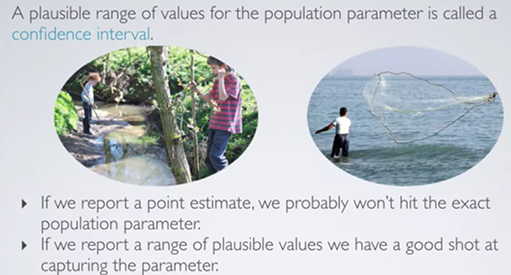
\includegraphics[width=0.8\linewidth]{graphs/2-3} 

}

\caption{Confidence interval}\label{fig:fig2-1}
\end{figure}

\section{Margin of Error}\label{margin-of-error}

margin of error = range一半对应的计量(若干个se)

\begin{figure}

{\centering 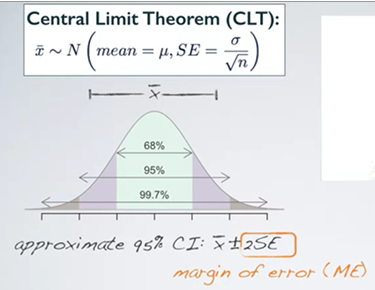
\includegraphics[width=0.8\linewidth]{graphs/2-4} 

}

\caption{Margin of error}\label{fig:fig2-4}
\end{figure}

例题1:

124情侣的研究表明,64.5\%的人喜欢在接吻的时候向右歪头,se为4\%

问下面说法那个错误:

\begin{figure}

{\centering 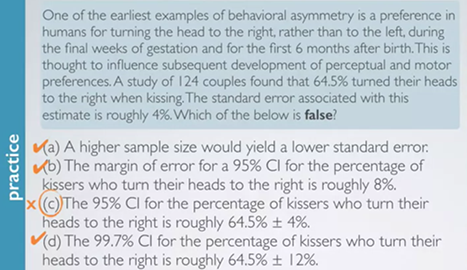
\includegraphics[width=0.8\linewidth]{graphs/2-5} 

}

\caption{Example}\label{fig:fig2-5}
\end{figure}

这里应该选C,因为95\%CI应该是64.5\%+/- 8\%,因为是加减2个SE

\begin{itemize}
\tightlist
\item
  margin of error = 1*se: 64.5\% confidential interval(CI)
\item
  margin of error = 2*se: 95\% CI
\item
  margin of error = 3*se: 99.7\% CI
\end{itemize}

\section{Confidential Interval}\label{confidential-interval}

Confidential interval for a population mean:

当我们知道了sample
mean的分布如何根据clt推导的时候,不需要进行多次sampling(用多组sample
来进行计算)

\begin{itemize}
\tightlist
\item
  在不知道population的standard deviation \texttt{σ}时,可以直接用这一组
  sample standard deviation \texttt{s} 来估\texttt{σ},然后
  用\(s/sqrt(n)\) 来估计standard error(即sample mean的standard
  deviation)
\item
  confidential interval: 这一组的sample mean加减 margin of error
  (z个se)
\end{itemize}

\begin{figure}

{\centering 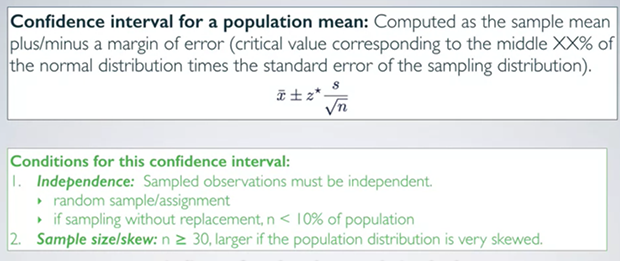
\includegraphics[width=0.8\linewidth]{graphs/2-6} 

}

\caption{Confidential Interval}\label{fig:fig2-6}
\end{figure}

注意这里的XX\% 表示的是这个distribution的middle部分的\%;
比如下图中想表达95\% confidence level,因此对应的是中间的95\%部分

\begin{figure}

{\centering 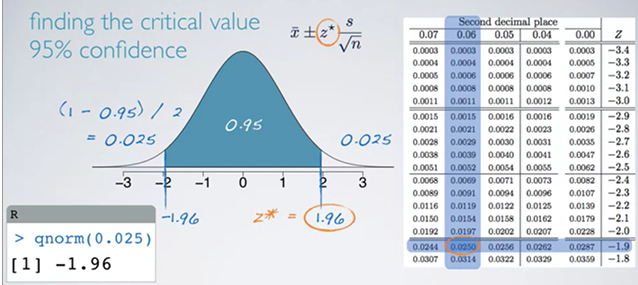
\includegraphics[width=0.8\linewidth]{graphs/2-7} 

}

\caption{Confidential Interval}\label{fig:fig2-7}
\end{figure}

在判断95\% confidence level的时候,往往会用X的平均值+/-两个SE

这里其实并不严谨。严格来说,应该是1.96个SE

这里1.96是通过先计算得到未被覆盖的部分占总distribution的0.025,然后用这个0.025到表中(或用左下角的R
function)找到对应的值-1.96,但由于是中心对称的,所以临界值其实对应的是正负1.96.

通常将正数的对应值成为critical value,也就是1.96.

\begin{Shaded}
\begin{Highlighting}[]
\KeywordTok{qnorm}\NormalTok{(}\FloatTok{0.025}\NormalTok{)}
\end{Highlighting}
\end{Shaded}

\begin{verbatim}
## [1] -1.959964
\end{verbatim}

\begin{Shaded}
\begin{Highlighting}[]
\KeywordTok{qnorm}\NormalTok{(}\DecValTok{1}\OperatorTok{-}\FloatTok{0.025}\NormalTok{)}
\end{Highlighting}
\end{Shaded}

\begin{verbatim}
## [1] 1.959964
\end{verbatim}

\section{Confidence Level}\label{confidence-level}

\textbf{confidence level}

\begin{itemize}
\tightlist
\item
  如果做很多次sampling(每次固定observation个数),然后取其confidence
  interval
\item
  有多少比重的sample可以contain 真正的population mean
\end{itemize}

\begin{figure}

{\centering 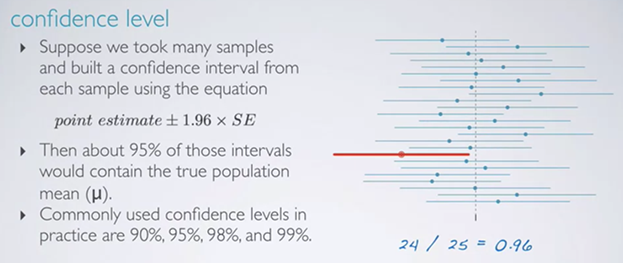
\includegraphics[width=0.8\linewidth]{graphs/2-8} 

}

\caption{Confidential Interval}\label{fig:fig2-8}
\end{figure}

\textbf{Accuracy}

\begin{itemize}
\tightlist
\item
  定义: whether or not the confidence interval contains the true
  population parameter.
\item
  例子: 这里假设取样25次,基于每次基于每个sample计算出对应的confidence
  interval,最后有24次都包含the true population
  mean(就是那个垂直的线),这样就可以计算accuracy为24/25=0.96
\item
  如果我们测试足够多次数的sample,最后会得到the percentage of capturing
  the true population parameter 为95\%
\item
  常用的confidence level为90\%,95\%,98\%,99\%
\end{itemize}

\textbf{Precision}

\begin{itemize}
\item
  定义: how small is the width of a confidence interval
\item
  当confidence level越大,interval就越宽
\end{itemize}

\begin{quote}
The higher the confidence level, the larger the critical value, hence
the larger the margin of error, and hence the width of the confidence
interval.
\end{quote}

\begin{figure}

{\centering 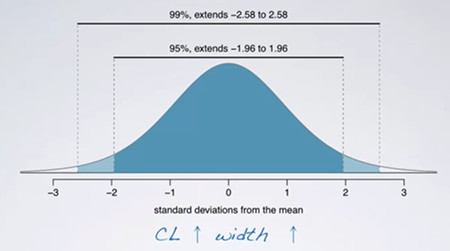
\includegraphics[width=0.8\linewidth]{graphs/2-9} 

}

\caption{Confidential level}\label{fig:fig2-9}
\end{figure}

\begin{itemize}
\tightlist
\item
  Interval 越宽,precision 越小
\end{itemize}

用一个比较wider
interval的缺点是,不够precise,不够informative,就像这个例子中,如果告诉你明天的温度是-29到43°之间,accuracy一定很高,但是意义不大;

\begin{figure}

{\centering 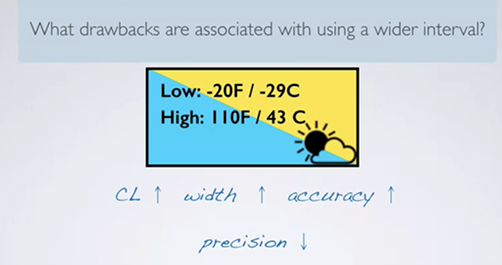
\includegraphics[width=0.8\linewidth]{graphs/2-10} 

}

\caption{Precision}\label{fig:fig2-10}
\end{figure}

\begin{itemize}
\tightlist
\item
  如何 同时增加precision(缩小range) 和 accuracy : \textbf{增加sample
  size}
\end{itemize}

因为sample size变大,standard
error变小,从而保证interval的width不会太宽,precision就不会因为accuracy上升而下降太多

\begin{itemize}
\tightlist
\item
  例题:
\end{itemize}

针对1154 美国居民调查,95\% confidence interval for the average
娱乐时间是3.53-3.73小时

\begin{figure}

{\centering 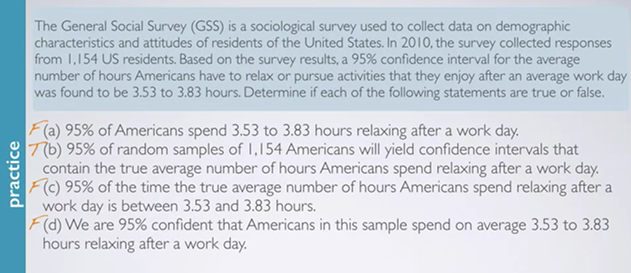
\includegraphics[width=0.8\linewidth]{graphs/2-11} 

}

\caption{Example 2}\label{fig:fig2-11}
\end{figure}

\begin{itemize}
\tightlist
\item
  A 不对是因为没有提到是基于sample中的结果,confidence
  interval并不是关于population中的individual的,而是关于the true
  population parameter (如population mean)的
\item
  B就很好,解释了有95\%的Confidence interval认为包含true population mean
\item
  C错是在于,true population
  parameter是一个定值,不是一个会一会在interval一会不在interval的moving
  target
\item
  D(最容易选错)错在,confidence interval不是关于sample
  mean的,而是关于population
  mean;除此之外,这个选项说有95\%的confidence认为sample
  mean在3.53到3.83之间,但其实应该是100\%,因为条件中表明了confidence
  level是这两个数,表明这两个数是sample
  mean的distribution的一部分,即这两个数一定是在这个区间内的。因此错
\end{itemize}

\section{Required sample size for margin of
error}\label{required-sample-size-for-margin-of-error}

据以下条件,我们可以算得desired margin of error 所需要的sample size:

\begin{itemize}
\tightlist
\item
  target margin of error
\item
  confidence level
\item
  variability of the sample/population
\end{itemize}

其他条件不变的情况下,sample size越大,margin of error越小

\begin{figure}

{\centering 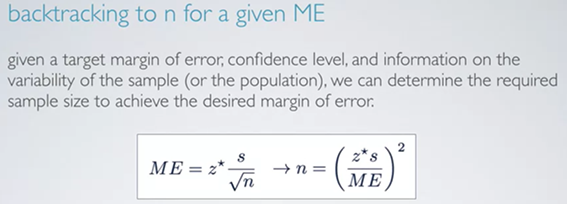
\includegraphics[width=0.8\linewidth]{graphs/2-12} 

}

\caption{A given ME}\label{fig:fig2-12}
\end{figure}

\section{Exercises}\label{exercises}

\begin{itemize}
\tightlist
\item
  例题(1)
\end{itemize}

三岁小孩的IQ的SD:18分

问: sample要多大才能obtain 90\% confidence interval with a margin of
error \textless{}= 4 points?

代入公式: z* 18/sqrt(n) = 4

\begin{figure}

{\centering 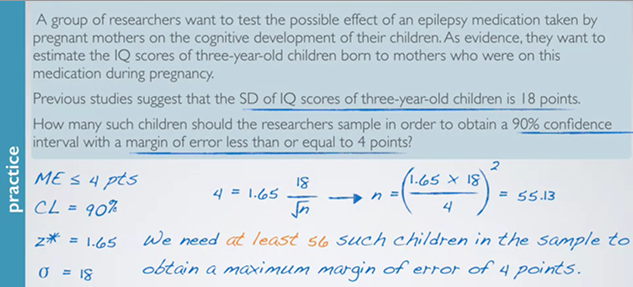
\includegraphics[width=0.8\linewidth]{graphs/2-13} 

}

\caption{Exercise 1}\label{fig:fig2-13}
\end{figure}

答: at least 55 samples

\begin{Shaded}
\begin{Highlighting}[]
\CommentTok{# 5%-95%}
\NormalTok{(z <-}\StringTok{  }\KeywordTok{qnorm}\NormalTok{(}\DecValTok{1}\OperatorTok{-}\FloatTok{0.05}\NormalTok{))}
\end{Highlighting}
\end{Shaded}

\begin{verbatim}
## [1] 1.644854
\end{verbatim}

\begin{Shaded}
\begin{Highlighting}[]
\NormalTok{(z}\OperatorTok{*}\DecValTok{18}\OperatorTok{/}\DecValTok{4}\NormalTok{)}\OperatorTok{**}\DecValTok{2}
\end{Highlighting}
\end{Shaded}

\begin{verbatim}
## [1] 54.78725
\end{verbatim}

\begin{itemize}
\tightlist
\item
  例题(2)
\end{itemize}

那如果我们要将margin of error降至2分,要如何变动sample size?

ME=z*sd/sqrt(n)

当ME下降一倍,sqrt(n)增加一倍,n增加四倍

\begin{figure}

{\centering 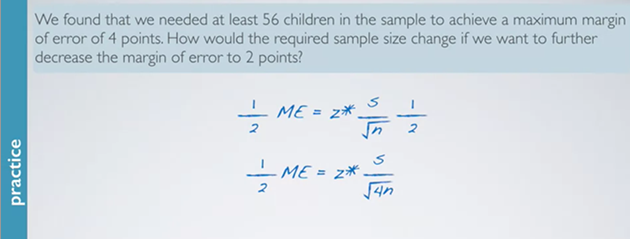
\includegraphics[width=0.8\linewidth]{graphs/2-14} 

}

\caption{Exercise 2}\label{fig:fig2-14}
\end{figure}

\begin{itemize}
\tightlist
\item
  类似,问:如果让interval 下降为1/3,要如何调整n?
\end{itemize}

答:interval的大小其实就是2倍的margin of error(ME),
让ME为1/3,即要求sqrt(n)增加3倍,那么n就要增加9倍

\begin{figure}

{\centering 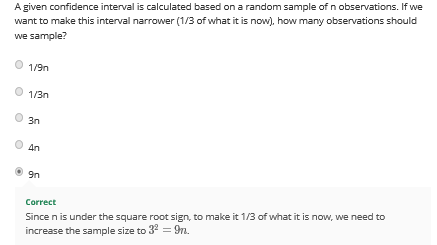
\includegraphics[width=0.8\linewidth]{graphs/2-15} 

}

\caption{Exercise 3}\label{fig:fig2-15}
\end{figure}

\begin{itemize}
\tightlist
\item
  例题 3
\end{itemize}

基于1151人数据,人们在过去30天中,会有95\% confidence interval of
3.40-4.24天感觉不开心

问:如何解释这里的interval

(答案如下)

\begin{figure}

{\centering 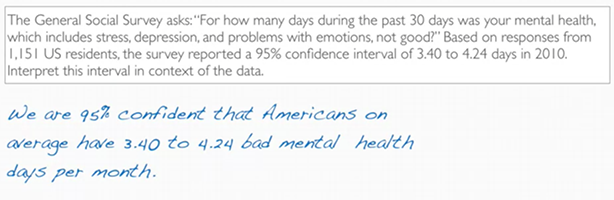
\includegraphics[width=0.8\linewidth]{graphs/2-16} 

}

\caption{Exercise 3}\label{fig:fig2-16}
\end{figure}

\begin{itemize}
\item
  confidence interval (CI)== point estimate +- margin of error
\item
  CI 是关于 unknown population mean的
\item
  CI (95\%), tells us how confident we are, \textbf{that this particular
  interval captures that mean}
\item
  例题4
\end{itemize}

50个sample学生显示,sample
mean是3.2个亲密关系的人,SD是1.74个,这里的sample dist有点skewed to the
right

问:estimate true average based on this sample using 95\% CI

答:

我们可以用CLT:

\begin{itemize}
\tightlist
\item
  这里因为sample数(50)\textgreater{}30 且 只是slightly
  skewed,可以assume the sampling distribution of average number 是nearly
  normal
\item
  50学生,我们假设\textgreater{}10\%,所以符合independent
\item
  sample是random selected
\end{itemize}

ME = z*SD/sqrt(n)

\begin{Shaded}
\begin{Highlighting}[]
\CommentTok{# 2.5%-97.5%}
\NormalTok{sd=}\FloatTok{1.74}
\NormalTok{n=}\DecValTok{50}
\NormalTok{z=}\KeywordTok{qnorm}\NormalTok{(}\DecValTok{1}\OperatorTok{-}\FloatTok{0.025}\NormalTok{)}
\NormalTok{sample_mean=}\FloatTok{3.2}
\NormalTok{(ME <-}\StringTok{ }\NormalTok{z}\OperatorTok{*}\NormalTok{sd}\OperatorTok{/}\NormalTok{(n}\OperatorTok{**}\NormalTok{(}\DecValTok{1}\OperatorTok{/}\DecValTok{2}\NormalTok{)))}
\end{Highlighting}
\end{Shaded}

\begin{verbatim}
## [1] 0.4822945
\end{verbatim}

\begin{Shaded}
\begin{Highlighting}[]
\KeywordTok{print}\NormalTok{(}\KeywordTok{paste}\NormalTok{(}\StringTok{"confidence interval:"}\NormalTok{,sample_mean}\OperatorTok{-}\NormalTok{ME,}\StringTok{"~"}\NormalTok{,sample_mean}\OperatorTok{+}\NormalTok{ME))}
\end{Highlighting}
\end{Shaded}

\begin{verbatim}
## [1] "confidence interval: 2.71770546912631 ~ 3.68229453087369"
\end{verbatim}

\begin{figure}

{\centering 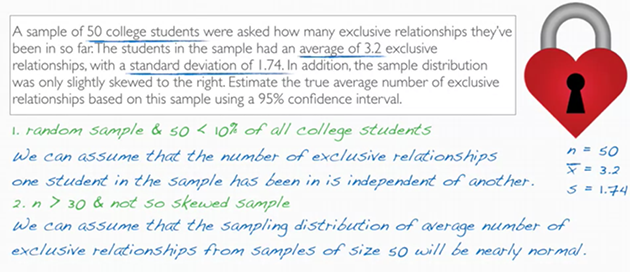
\includegraphics[width=0.8\linewidth]{graphs/2-17} 

}

\caption{Exercise 4}\label{fig:fig2-171}
\end{figure}\begin{figure}

{\centering 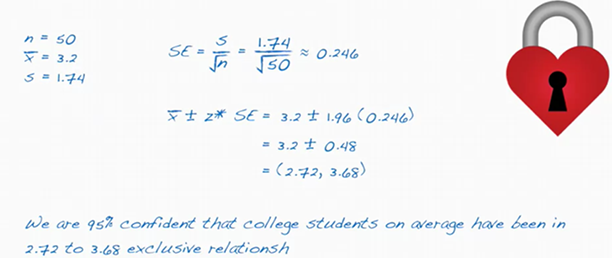
\includegraphics[width=0.8\linewidth]{graphs/2-18} 

}

\caption{Exercise 4}\label{fig:fig2-172}
\end{figure}

\begin{itemize}
\tightlist
\item
  例题5
\end{itemize}

random sample: 100 runners, 跑完10mile的平均速度是95 min,95\%
CI是92min-98min,问下面哪个不对:

注意下面2中正确的说法应该是:

\begin{quote}
CI: we are XX\% confident that the true population parameter is in this
interval
\end{quote}

\begin{figure}

{\centering 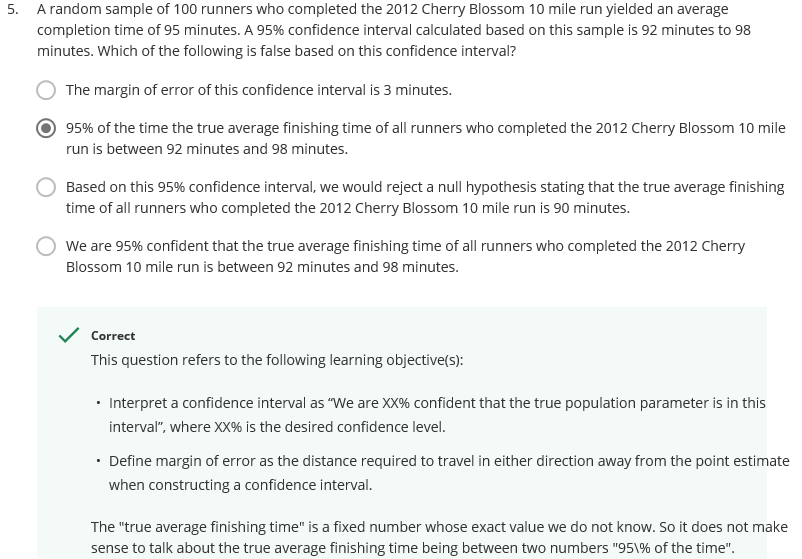
\includegraphics[width=0.8\linewidth]{graphs/2-19} 

}

\caption{Exercise 5}\label{fig:fig2-19}
\end{figure}

\chapter{Hypothesis Testing}\label{test}

\section{Chapter Summary}\label{chapter-summary}

\begin{figure}

{\centering 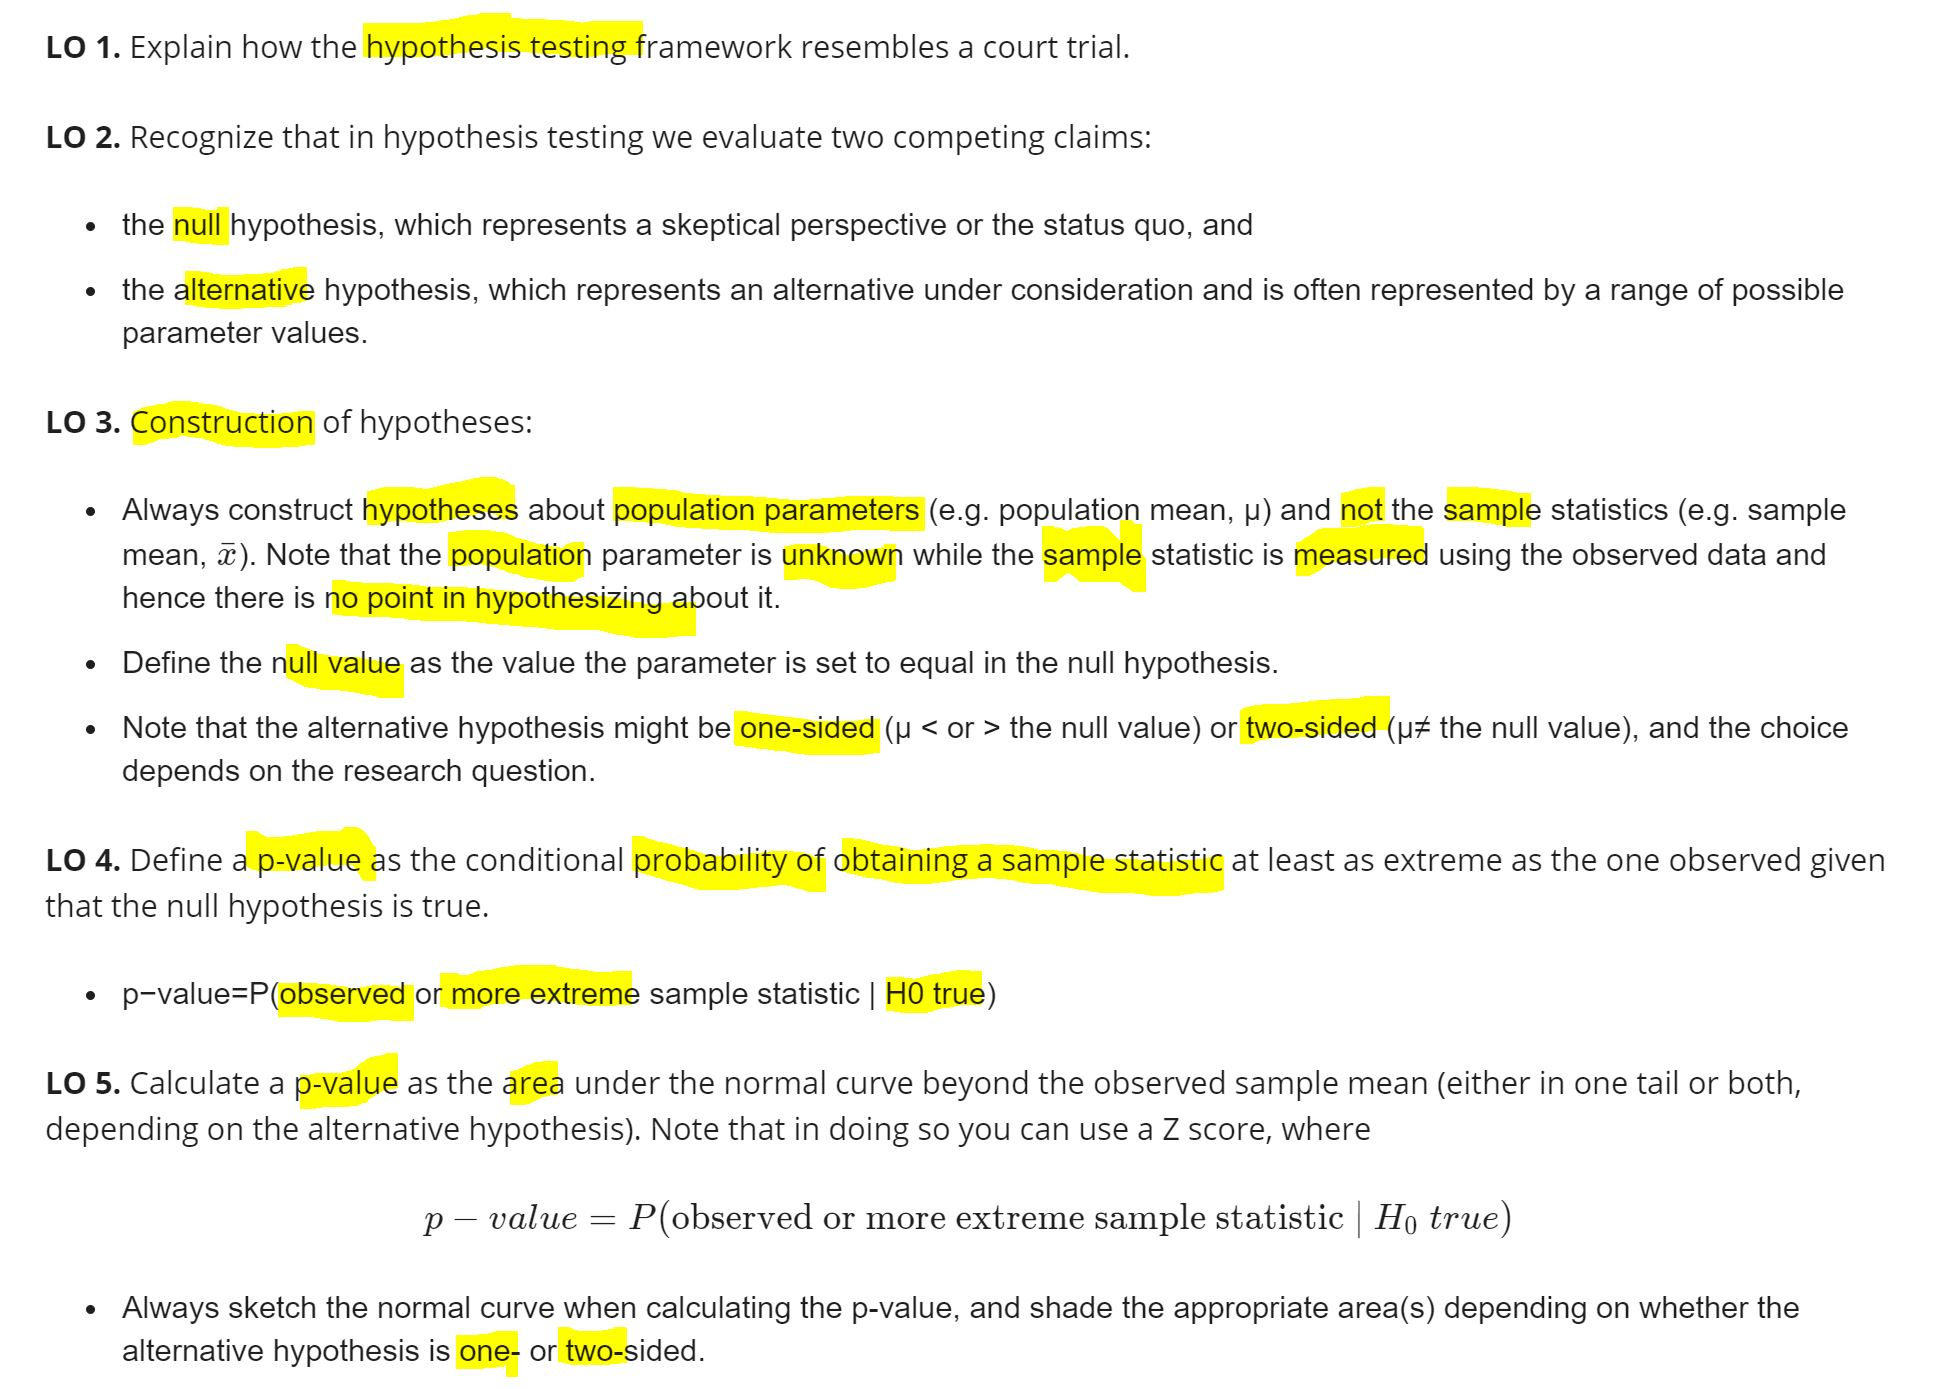
\includegraphics[width=0.8\linewidth]{graphs/3-1} 

}

\caption{Chapter Summary}\label{fig:chap3-summary-fig1}
\end{figure}\begin{figure}

{\centering 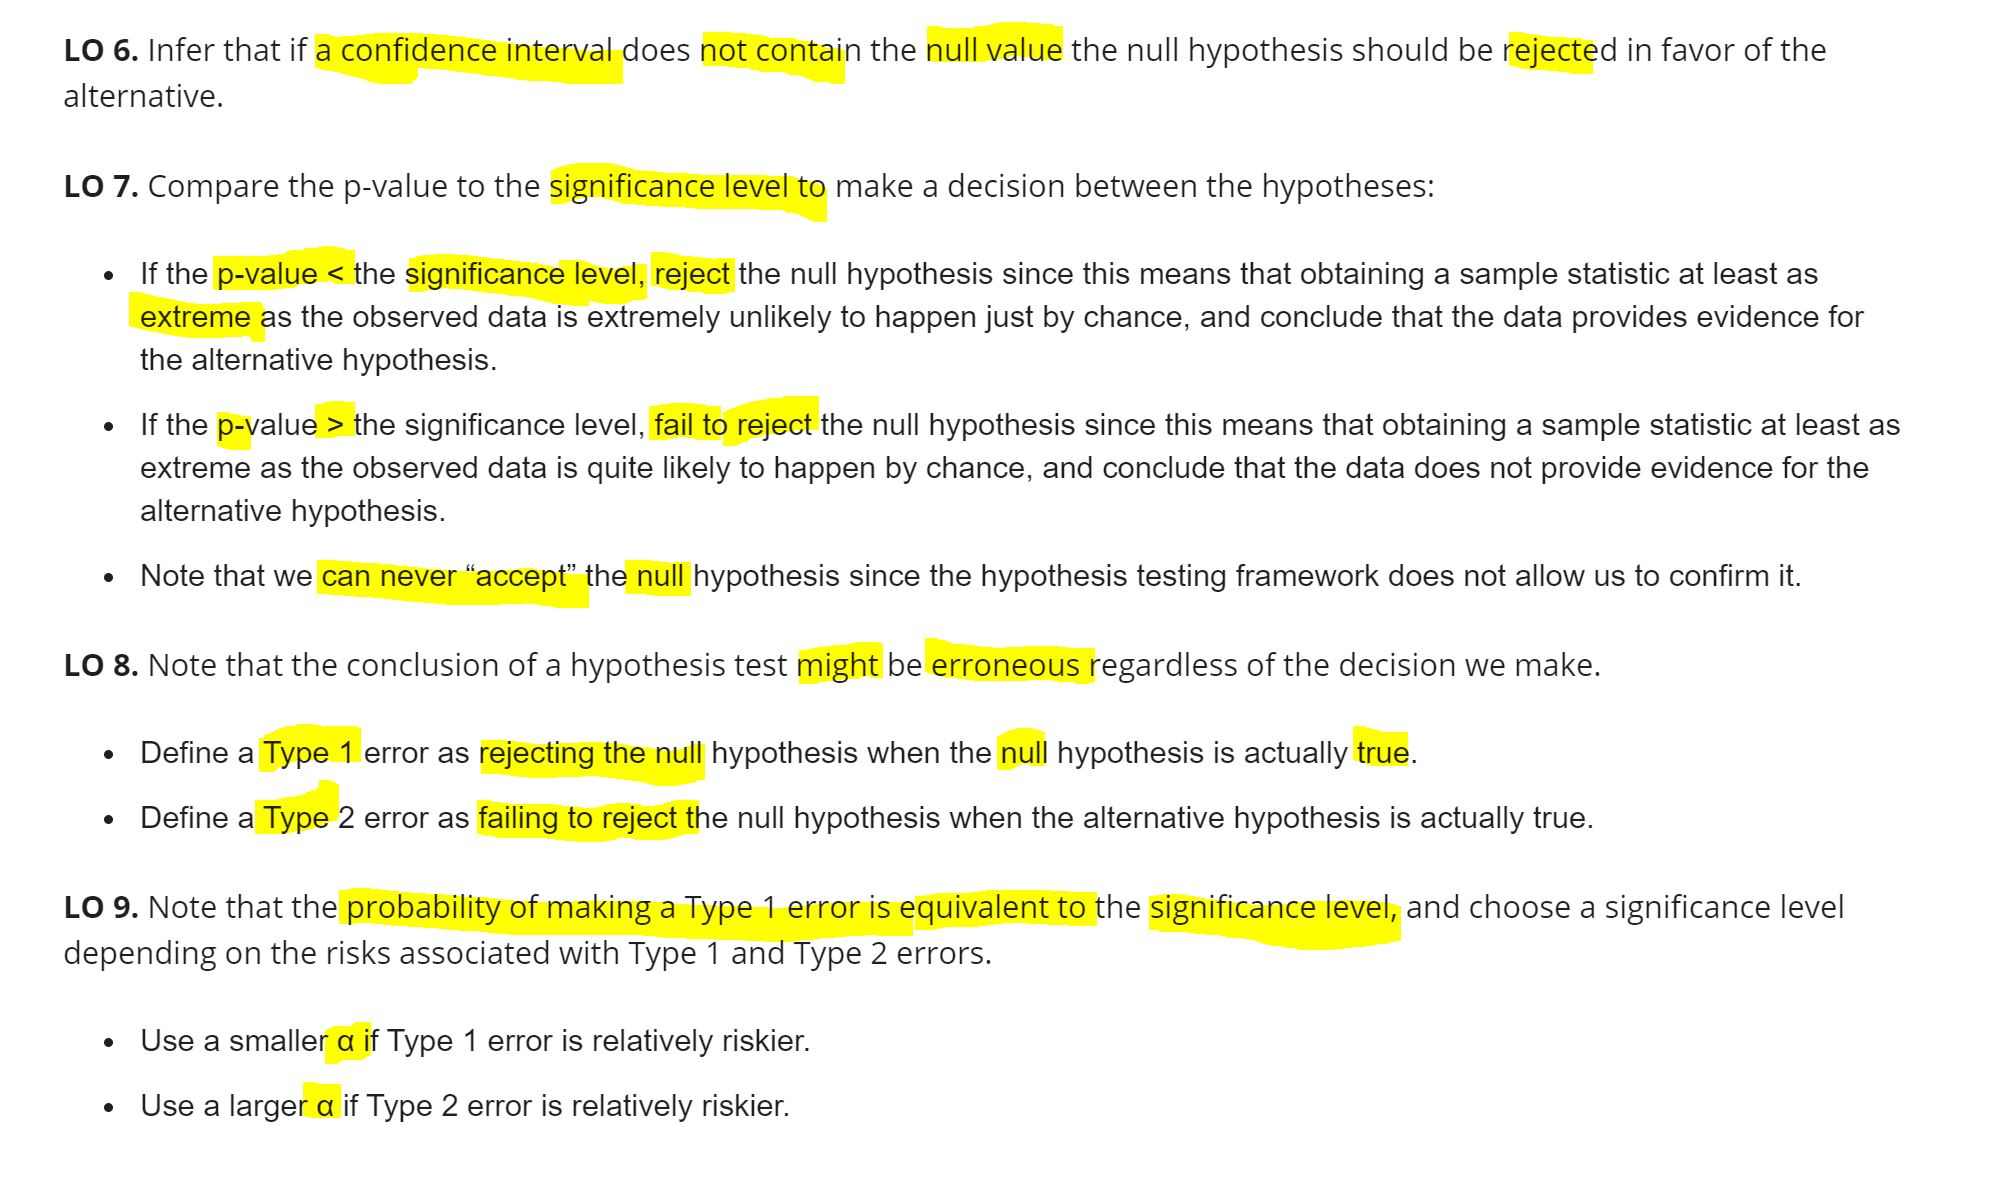
\includegraphics[width=0.8\linewidth]{graphs/3-2} 

}

\caption{Chapter Summary}\label{fig:chap3-summary-fig2}
\end{figure}

\chapter{Applications}\label{applications}

Some \emph{significant} applications are demonstrated in this chapter.

\section{Example one}\label{example-one}

\section{Example two}\label{example-two}

\chapter{Final Words}\label{final-words}

We have finished a nice book.

\bibliography{book.bib,packages.bib}

\end{document}
